
%%%%%%%%%%%%%%%%%%%%%%%%%%%%%%%%%%%%%%%%%%%%%%%%%%%%%%
\begin{frame}[c]{ }
	\frametitle{Hadoop Core Concepts }
	
	
	\begin{itemize}  [<+->]
		\item [--] HDFS.
		\item [--] YARN.
		\item [--] Map-Reduce.
		
	\end{itemize}
\end{frame}
%%%%%%%%%%%%%%%%%%%%%%%%%%%%%%%%%%%%%%%%%%%%%%%%%%%%%%
\begin{frame}[c]{ }
	\frametitle{ Hadoop Map Reduce}
	\centering     
	
	\textcolor{offgreen}{ \large Introduction To Hadoop Map Reduce API}
\end{frame}
%%%%%%%%%%%%%%%%%%%%%%%%%%%%%%%%%%%%%%%%%%%%%%%%%%%%%%	

\begin{frame}
\frametitle{The basic idea of MapReduce}
We break this into three stages
\begin{itemize}  [<+->]
	\item Map.
	\item Shuffle/Group (Mapper Intermediates).
	\item Reduce			
\end{itemize}
\footnotetext[1]{This example taken from  \href{https://reberhardt.com/cs110/summer-2018/lecture-notes/lecture-14/}{https://reberhardt.com/cs110/summer-2018/lecture-notes/lecture-14/}	} 
\end{frame}
%%%%%%%%%%%%%%%%%%%%%%%%%%%%%%%%%%%%%%%%%%%%%%%%%%%%%%
\begin{frame}
\frametitle{Map}
We distribute our raw ingredients amongst the workers.
\begin{figure}
	\includegraphics[width=.5\textwidth,height=.7\textheight]{./Figures/chapter-02/map-reduce-map-side.jpeg}
\end{figure}			
\footnotetext[1]{{\tiny This example taken from  \href{https://reberhardt.com/cs110/summer-2018/lecture-notes/lecture-14/}{https://reberhardt.com/cs110/summer-2018/lecture-notes/lecture-14/}	} }
\end{frame}
%%%%%%%%%%%%%%%%%%%%%%%%%%%%%%%%%%%%%%%%%%%%%%%%%%%%%%
\begin{frame}
\frametitle{Shuffle/Group}
We will organise and group the processed ingredients into piles, so that making a sandwich becomes easy.
\begin{figure}
	\includegraphics[width=.7\textwidth,height=.64\textheight]{./Figures/chapter-02/map-reduce-shuffle.png}
\end{figure}			
\footnotetext[1]{{\tiny This example taken from  \href{https://reberhardt.com/cs110/summer-2018/lecture-notes/lecture-14/}{https://reberhardt.com/cs110/summer-2018/lecture-notes/lecture-14/}	}} 
\end{frame}
%%%%%%%%%%%%%%%%%%%%%%%%%%%%%%%%%%%%%%%%%%%%%%%%%%%%%%
\begin{frame}
\frametitle{Reduce}
we’ll combine the ingredients into a sandwich
\begin{figure}
	\includegraphics[width=.96\textwidth,height=.7\textheight]{./Figures/chapter-02/map-reduce-reduce-side.png}
\end{figure}			
\footnotetext[1]{ {\tiny This example taken from  \href{https://reberhardt.com/cs110/summer-2018/lecture-notes/lecture-14/}{https://reberhardt.com/cs110/summer-2018/lecture-notes/lecture-14/}	}} 
\end{frame}
%%%%%%%%%%%%%%%%%%%%%%%%%%%%%%%%%%%%%%%%%%%%%%%%%%%%%%
\begin{frame}[plain,c]
	\frametitle{Case Study Example 1}
	\begin{figure}
		\centering
		\input{./Figures/chapter-02/ds_case_study_1_1.tex}
		\caption{Convert text to upper text, for example, The -> THE } \label{fig:DS3}
	\end{figure}
	
\end{frame}
%%%%%%%%%%%%%%%%%%%%%%%%%%%%%%%%%%%%%%%%%%%%%%%%%%%%%%
\begin{frame}[plain,c]
	\frametitle{Case Study Example 1}
	\begin{figure}
		\centering
		\input{./Figures/chapter-02/ds_case_study_1_3.tex}
	\end{figure}


\end{frame}

%%%%%%%%%%%%%%%%%%%%%%%%%%%%%%%%%%%%%%%%%%%%%%%%%%%%%%
\begin{frame}[plain,c]
	\frametitle{Case Study Example 2}
	\begin{figure}
		\centering
		\input{./Figures/chapter-02/ds_case_study_2_1.tex}
	\end{figure}
	
\end{frame}

%%%%%%%%%%%%%%%%%%%%%%%%%%%%%%%%%%%%%%%%%%%%%%%%%%%%%%
\begin{frame}

	\begin{figure}
		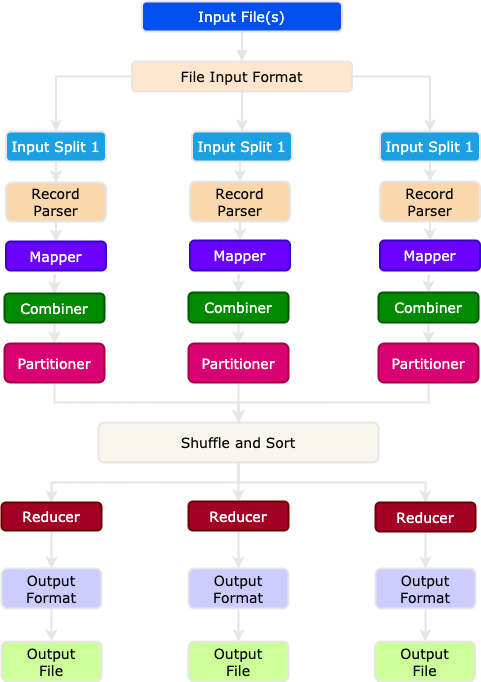
\includegraphics[height=.925\textheight]{./Figures/chapter-02/Map-Reduce.png}
				\caption{Map Reduce Stages } \label{fig:MRSteps}
	\end{figure}			
\end{frame}
%%%%%%%%%%%%%%%%%%%%%%%%%%%%%%%%%%%%%%%%%%%%%%%%%%%%%%
\begin{frame}
	
	\begin{figure}
		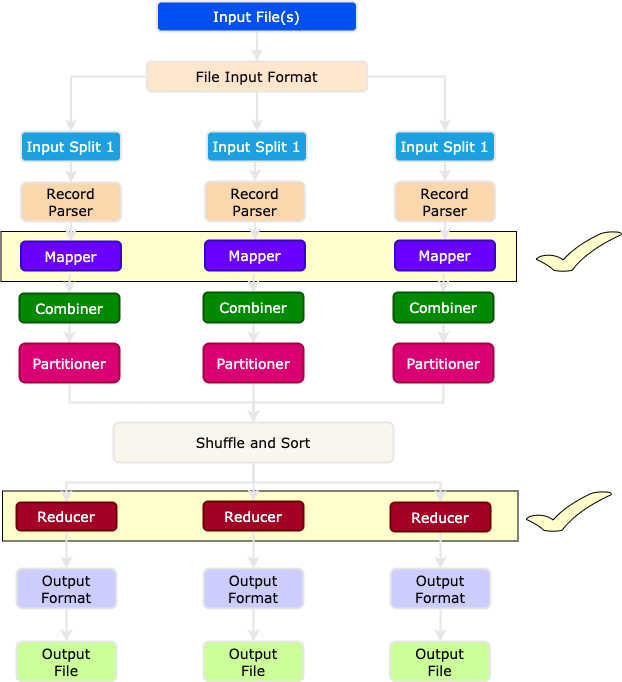
\includegraphics[height=.925\textheight]{./Figures/chapter-02/Map-Reduce_2.png}
		\caption{Map Reduce Stages } \label{fig:MRSteps2}
	\end{figure}			
\end{frame}
%%%%%%%%%%%%%%%%%%%%%%%%%%%%%%%%%%%%%%%%%%%%%%%%%%%%%%
\begin{frame}[c]{ }
	\frametitle{Map Reduce (word count) Deep Dive }
	
	The Map-Reduce consists of three "main" parts
	
	\begin{itemize}  [<+->]
		\item [--] The Driver.
		\item [--] The Mapper.
		\item [--] The Reducer.
		
	\end{itemize}
\end{frame}
%%%%%%%%%%%%%%%%%%%%%%%%%%%%%%%%%%%%%%%%%%%%%%%%%%%%%%
\begin{frame}[c]{ }
	\frametitle{ Hadoop Map Reduce API}
	\centering     
	
	\textcolor{offgreen}{ \large Hadoop Map Reduce API Deep Dive}
\end{frame}
%%%%%%%%%%%%%%%%%%%%%%%%%%%%%%%%%%%%%%%%%%%%%%%%%%%%%%
\begin{frame}[c]{ }
	\frametitle{The Driver }

	\begin{itemize}  [<+->]
		\item [--] The code that runs on the client machine configures the job details by creating an object from the \code{Job}  class, which implements the \code{JobContext} interface.
		\item [--] It submits the job to the cluster.		
		\item [--] It parses job arguments to identify job parameters, for example, input/output directories.. 
		
	\end{itemize}

\end{frame}
%%%%%%%%%%%%%%%%%%%%%%%%%%%%%%%%%%%%%%%%%%%%%%%%%%%%%%
\begin{frame}[c]{ }
	\frametitle{The Driver:  Job Configuration}
	

The \code{Job}  object allows you to set configuration for your \code{Map-Reduce} job:
			\begin{itemize}  [<+->]
				\item [--] You can configure the \code{Mapper} \& the \code{Reducer} classes.
				\item [--] Set the \code{Mapper} input/output key \& value data types.
				\item [--] Set the \code{Reducer} input/output key \& value data types.
	
		
			\end{itemize}		

	
\end{frame}
%%%%%%%%%%%%%%%%%%%%%%%%%%%%%%%%%%%%%%%%%%%%%%%%%%%%%%
\begin{frame}[c]{ }
	\frametitle{The Driver:  Job Configuration}
	
	\begin{itemize}  [<+->]
		\item [--] We can configure file input directory and output.
		\item [--] We configure the output path using \code{FileOutputFormat.setOutputPath()} to specify the reducers' directory to write the output data.
	\end{itemize}		
	
\end{frame}
%%%%%%%%%%%%%%%%%%%%%%%%%%%%%%%%%%%%%%%%%%%%%%%%%%%%%%
\begin{frame}[c]{ }
	\frametitle{The Driver:  Job Configuration}
	
	\begin{itemize}  [<+->]
		\item [--] We configure the input path using \code{FileInputFormat.setInputPaths()}, and by default, it will read all the files in the specified directories and send them to the mappers.
		
		\item [--] We can use \code{Hadoop glob patterns} to read directory patterns, for example, \textit{/warehouse/public/sales*}.
		\item [--] We can call \code{FileInputFormat.addInputPath()} to multiple times by specifying a single file or directory. 
		
	\end{itemize}		
	
	\footnotetext[1]{For more details, please read HTDG. Ch.3 File patterns and PathFilter sections.	} 
\end{frame}
%%%%%%%%%%%%%%%%%%%%%%%%%%%%%%%%%%%%%%%%%%%%%%%%%%%%%%
\begin{frame}[c]{ }
	\frametitle{ Hadoop Map Reduce API}
	\centering     
	
	\textcolor{offgreen}{ \large Please read HTDG. Ch.3 The Java Interface}
\end{frame}
%%%%%%%%%%%%%%%%%%%%%%%%%%%%%%%%%%%%%%%%%%%%%%%%%%%%%%


\begin{frame}[c]{ }
	\frametitle{The Driver:  Job Configuration }
	
		
		\begin{itemize}  [<+->]

			\item [--] You could set driver configurations globally using Hadoop configurations.
			\item [--] Any options not specified in the job configuration will use the Hadoop default values.
			\item [--] We use the \code{Job} object to specify the job name and check its state..
		
			
	\end{itemize}
	
\end{frame}
%%%%%%%%%%%%%%%%%%%%%%%%%%%%%%%%%%%%%%%%%%%%%%%%%%%%%%
\begin{frame}[c]{ }
	\frametitle{The Driver:  Job Configuration }
	

	\begin{itemize}  [<+->]
		
	\item [--] It is optional to set the mapper and reducer classes.
	\item [--] Hadoop uses its default \code{IdentityMapper} and \code{IdentityReducer}.		
		
	\end{itemize}
	
\end{frame}
%%%%%%%%%%%%%%%%%%%%%%%%%%%%%%%%%%%%%%%%%%%%%%%%%%%%%%
\begin{frame}[c]{ }
	\frametitle{The Driver:  Job Configuration }
	
	
	Lunch a Map-Reduce job:
	\begin{itemize}  [<+->]
		
		\item [--] The \code{waitForCompletion()} method in the \code{Job} class launches the job and polls for progress. In addition, it writes the logs and summarizing the Map-Reduce job progress and changes.

	\item [--] When the job completes successfully, the job counters are displayed. Otherwise, the error that caused the job to fail is logged to the console.
		
	\end{itemize}
	
\end{frame}
%%%%%%%%%%%%%%%%%%%%%%%%%%%%%%%%%%%%%%%%%%%%%%%%%%%%%%
\begin{frame}[c]{ }
	\frametitle{InputFormat}
	
	\begin{itemize}  [<+->]
		\item [--] TheThe driver defines the \code{InputFormat}; then the \code{InputFormat} creates a \code{RecordReader"} object that parses the input data into key/value pairs passed to the mapper.
		\item [--] For example: \code{TextInputFormat}:
		\begin{itemize}  [<+->]
			
			\item It is the default.
			\item It creates \code{LineRecordReader} objects.
			\item Key: is the line offest in the file.
			\item Value: is the line which terminated by "\textbackslash n".
		\end{itemize}		
		
		
	\end{itemize}		
	
\end{frame}
%%%%%%%%%%%%%%%%%%%%%%%%%%%%%%%%%%%%%%%%%%%%%%%%%%%%%%
\begin{frame}[c]{ }
	\frametitle{Keys and Values}
	
	\begin{itemize}  [<+->]
		\item [--] Keys and Values in Hadoop are java \code{Objects} not \code{Java primitives types}.
		\item [--] Values are objects which implement \code{Writable}.
		\item [--] Keys are objects which implement \code{WritableComparable}.

		
	\end{itemize}		
	
\end{frame}
%%%%%%%%%%%%%%%%%%%%%%%%%%%%%%%%%%%%%%%%%%%%%%%%%%%%%%
\begin{frame}[c]{ }
	\frametitle{What is Writable?}
	
	\begin{itemize}  [<+->]
		\item [--] \code{Writable} is an interface in Hadoop.
		\item [--] \code{Writables} are used for data type "serialization" in Hadoop to translate/serialize "primitive java data types" to "Hadoop data types", Ex: int to IntWritable and String to Text.
		\item [--] Hadoop uses the \code{Writable} interface for data transfer in the cluster and network.
		
		
	\end{itemize}		
	
\end{frame}
%%%%%%%%%%%%%%%%%%%%%%%%%%%%%%%%%%%%%%%%%%%%%%%%%%%%%%
\begin{frame}[c]{ }
	\frametitle{What is WritableComparable?}
	
	\begin{itemize}  [<+->]
		\item [--] A \code{WritableComparable} is a \code{Writable} which is also \code{Comparable}.
		\item [--] We can compare two \code{WritableComparables} against each other to determine their \textbf{\underline{\textit{order}}}, for example, we could need to compare the order of two Text "Apple vs. Cat or numbers ordering" to understand the ordering mechanism. 
		\item [--] Obviously, the reason we have Keys to be \code{WritableComparable} is that they are passed to the reducer in \underline{\textit{\textbf{sorted order}}}.
		\item [--] Note: All Hadoop implemented types are both \code{Writable} and \code{WritableComparable}.
		
		
	\end{itemize}		
	
\end{frame}
%%%%%%%%%%%%%%%%%%%%%%%%%%%%%%%%%%%%%%%%%%%%%%%%%%%%%%
\begin{frame}[c]{ }
	\frametitle{Map Reduce (word count) Deep Dive }
	
	The Map-Reduce example consists of three main parts
	
	\begin{itemize}  [<+->]
		\item [--] \sout{The Driver}.
		\item [--] The Mapper.

		
	\end{itemize}
\end{frame}
%%%%%%%%%%%%%%%%%%%%%%%%%%%%%%%%%%%%%%%%%%%%%%%%%%%%%%
\begin{frame}[c]{ }
	\frametitle{The Mapper}
		
	\begin{itemize}  [<+->]
		
		\item [--] The mapper class deals with a single input split.
		
		\item [--] All mapper classes must extend the \code{Mapper} base class.

		\item [--] All mapper must specify the key and values for input and output.		
		
		\item [--] All mappers must override the \code{map} method and pass the key, value, and \code{Context}.
		
		\item [--]  The \code{Context} is used to write intermediate data and all information about the job's configurations.
		
	\end{itemize}
	
\end{frame}
%%%%%%%%%%%%%%%%%%%%%%%%%%%%%%%%%%%%%%%%%%%%%%%%%%%%%%
\begin{frame}[c]{ }
	\frametitle{Map Reduce (word count) Deep Dive }
	
	The Map-Reduce example consists of three main parts
	
	\begin{itemize}  [<+->]
		\item [--] \sout{The Driver}.
		\item [--] \sout{The Mapper}.
		\item [--] The Reducer.
		
	\end{itemize}
\end{frame}
%%%%%%%%%%%%%%%%%%%%%%%%%%%%%%%%%%%%%%%%%%%%%%%%%%%%%%
\begin{frame}[c]{ }
	\frametitle{The Reducer}
	
	\begin{itemize}  [<+->]
		
		\item [--] The Reducer receives a Key and an Iterable collection of Writable objects. It also receives a Context object.
		
		\item [--] All reducers classes must extend the  \code{Reducer} base class.
		
		\item [--] All mapper must specify the key and values for intermediate input and final (or intermediate) output.		
		
		\item [--] All reducers must override the "reduce" method and pass the key, \code{Iterable} and "Context".

	\end{itemize}
	
\end{frame}
%%%%%%%%%%%%%%%%%%%%%%%%%%%%%%%%%%%%%%%%%%%%%%%%%%%%%%
\begin{frame}[c]{ }
	\frametitle{ Hadoop Map Reduce API}
	\centering     
	
	\textcolor{offgreen}{ \large Map Reduce Demo}
\end{frame}
